\section{Construcción de la red}

Usando las herramientas ya mencionadas, se comenzó el proceso de recopilación de
la actividad, usando como filtro los \textit{hashtags} más usados en los
\textit{tweets} relativos al tema deseado: \textbf{\#PilarNosMiente},
\textbf{\#vergUGRenza} y \textbf{\#verUGRenza}.

La red que se ha descargado es del tipo \textit{Full Twitter network}, de forma
que contiene tanto \textit{tweets} como usuarios, \textit{hashtags}, enlaces y
contenido multimedia. Así, obtenemos toda la actividad relativa a este tema de
discusión.

El proceso de recopilación tuvo lugar del 5 al 8 de mayo, obteniendo con la
actividad de este período de tiempo la red de la Figura \ref{fig:full}. Se
trata, obviamente, de una red dirigida, con un total de 5764 nodos y 10718
enlaces. Los nodos representan los elementos ya indicados (\textit{tweets},
usuarios, \textit{hashtags}, enlaces y contenido multimedia), mientras que los
enlaces pueden representar diversas cosas dependiendo de los tipos de nodos que
conecten, siendo las más relevantes las siguientes:

\begin{itemize}
    \item Un usuario se conecta con otro al que hace \textit{retweet} o cita.
    \item Un usuario se conecta con un \textit{tweet} que publica, cita o al que
          hace \textit{retweet}.
    \item Un \textit{tweet} se conecta con un usuario al que menciona.
    \item Un \textit{tweet} se conecta con los \textit{hashtags}, enlaces y
          contenido multimedia que contiene.
\end{itemize}

En la Figura \ref{fig:full}, se han usado colores para reflejar el tipo de
elemento que representa cada nodo: los \textit{tweets} en rojo, los usuarios en
verde y el resto en gris. Estos últimos tipos se han puesto del mismo color dado
que representan tan solo el 2,89\% de los nodos de la red, lo que hace que sean
casi imperceptibles en la representación.

\begin{figure}
    \centering
    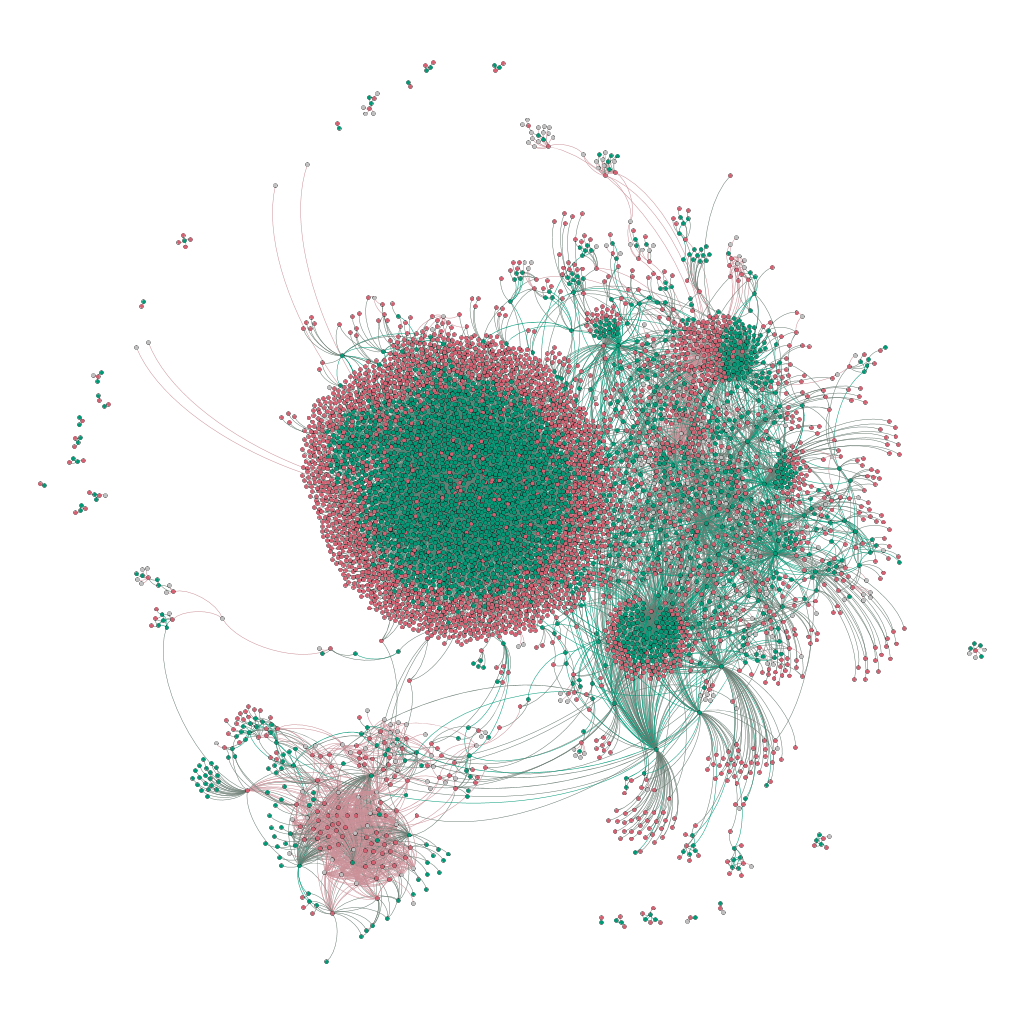
\includegraphics[width=\textwidth]{images/graph/full.png}
    \caption{Red completa con clasificación por colores de los elementos}
    \label{fig:full}
\end{figure}

La red obtenida es muy grande, por lo que he tenido que reducir su tamaño. Para
ello, he decidido eliminar todos los nodos que representan \textit{hashtags},
enlaces y contenido multimedia, debido a que son un porcentaje muy pequeño y
apenas aportan información valiosa. Además, he aplicado un filtro
\textit{k-core} con un valor de k de 2. De esta forma, me he quedado con una
cantidad final de 2970 nodos y 6705 enlaces. La red resultante es la de la
Figura \ref{fig:filtered}. Comparándola con la inicial, vemos como se han
eliminado casi todos los \textit{tweets} que se encontraban en la gran masa de
nodos central, ya que tenían grado 1.

\begin{figure}
    \centering
    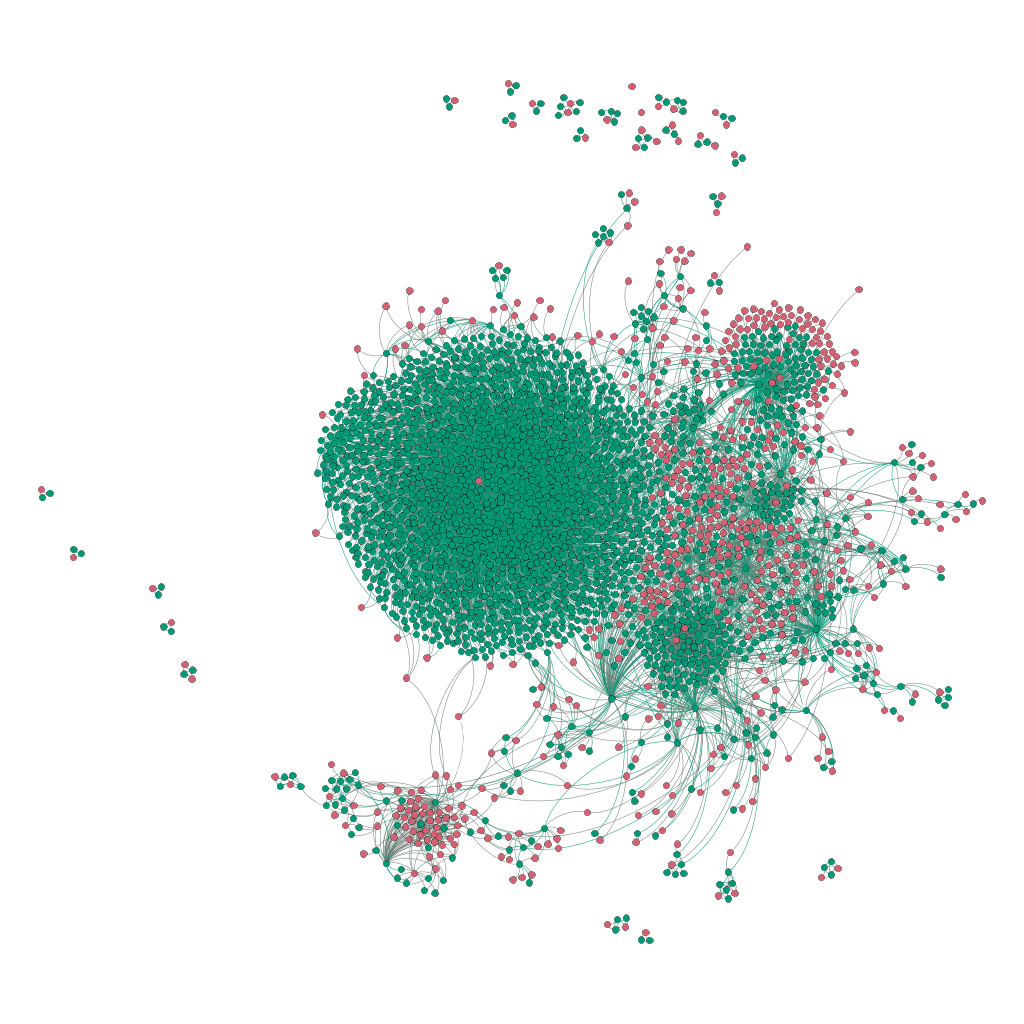
\includegraphics[width=\textwidth]{images/graph/filtered.png}
    \caption{Red filtrada de \textit{tweets} y usuarios representando el grado de los nodos por su tamaño}
    \label{fig:filtered}
\end{figure}
